% Created by tikzDevice version 0.12 on 2019-04-06 22:05:05
% !TEX encoding = UTF-8 Unicode
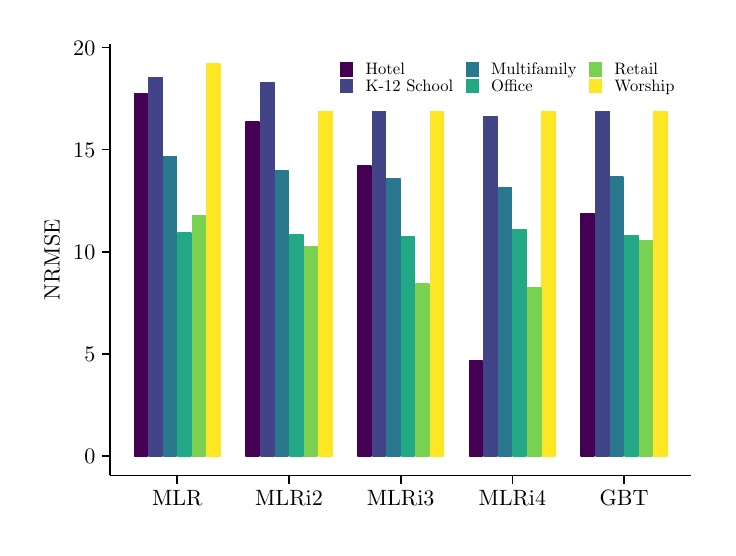
\begin{tikzpicture}[x=1pt,y=1pt]
\definecolor{fillColor}{RGB}{255,255,255}
\path[use as bounding box,fill=fillColor,fill opacity=0.00] (0,0) rectangle (245.72,180.67);
\begin{scope}
\path[clip] (  0.00,  0.00) rectangle (245.72,180.67);
\definecolor{drawColor}{RGB}{255,255,255}
\definecolor{fillColor}{RGB}{255,255,255}

\path[draw=drawColor,line width= 0.6pt,line join=round,line cap=round,fill=fillColor] (  0.00,  0.00) rectangle (245.72,180.68);
\end{scope}
\begin{scope}
\path[clip] ( 29.85, 18.85) rectangle (239.72,174.67);
\definecolor{fillColor}{RGB}{255,255,255}

\path[fill=fillColor] ( 29.85, 18.85) rectangle (239.72,174.67);
\definecolor{drawColor}{RGB}{253,231,37}
\definecolor{fillColor}{RGB}{253,231,37}

\path[draw=drawColor,line width= 0.6pt,line join=round,fill=fillColor] ( 64.83, 25.94) rectangle ( 69.54,167.59);
\definecolor{drawColor}{RGB}{122,209,81}
\definecolor{fillColor}{RGB}{122,209,81}

\path[draw=drawColor,line width= 0.6pt,line join=round,fill=fillColor] ( 59.58, 25.94) rectangle ( 64.29,112.52);
\definecolor{drawColor}{RGB}{34,168,132}
\definecolor{fillColor}{RGB}{34,168,132}

\path[draw=drawColor,line width= 0.6pt,line join=round,fill=fillColor] ( 54.34, 25.94) rectangle ( 59.04,106.36);
\definecolor{drawColor}{RGB}{42,120,142}
\definecolor{fillColor}{RGB}{42,120,142}

\path[draw=drawColor,line width= 0.6pt,line join=round,fill=fillColor] ( 49.09, 25.94) rectangle ( 53.80,134.06);
\definecolor{drawColor}{RGB}{65,68,135}
\definecolor{fillColor}{RGB}{65,68,135}

\path[draw=drawColor,line width= 0.6pt,line join=round,fill=fillColor] ( 43.84, 25.94) rectangle ( 48.55,162.61);
\definecolor{drawColor}{RGB}{68,1,84}
\definecolor{fillColor}{RGB}{68,1,84}

\path[draw=drawColor,line width= 0.6pt,line join=round,fill=fillColor] ( 38.60, 25.94) rectangle ( 43.30,156.63);
\definecolor{drawColor}{RGB}{253,231,37}
\definecolor{fillColor}{RGB}{253,231,37}

\path[draw=drawColor,line width= 0.6pt,line join=round,fill=fillColor] (105.19, 25.94) rectangle (109.90,163.87);
\definecolor{drawColor}{RGB}{122,209,81}
\definecolor{fillColor}{RGB}{122,209,81}

\path[draw=drawColor,line width= 0.6pt,line join=round,fill=fillColor] ( 99.94, 25.94) rectangle (104.65,101.60);
\definecolor{drawColor}{RGB}{34,168,132}
\definecolor{fillColor}{RGB}{34,168,132}

\path[draw=drawColor,line width= 0.6pt,line join=round,fill=fillColor] ( 94.70, 25.94) rectangle ( 99.40,105.66);
\definecolor{drawColor}{RGB}{42,120,142}
\definecolor{fillColor}{RGB}{42,120,142}

\path[draw=drawColor,line width= 0.6pt,line join=round,fill=fillColor] ( 89.45, 25.94) rectangle ( 94.16,129.06);
\definecolor{drawColor}{RGB}{65,68,135}
\definecolor{fillColor}{RGB}{65,68,135}

\path[draw=drawColor,line width= 0.6pt,line join=round,fill=fillColor] ( 84.20, 25.94) rectangle ( 88.91,160.87);
\definecolor{drawColor}{RGB}{68,1,84}
\definecolor{fillColor}{RGB}{68,1,84}

\path[draw=drawColor,line width= 0.6pt,line join=round,fill=fillColor] ( 78.96, 25.94) rectangle ( 83.66,146.48);
\definecolor{drawColor}{RGB}{253,231,37}
\definecolor{fillColor}{RGB}{253,231,37}

\path[draw=drawColor,line width= 0.6pt,line join=round,fill=fillColor] (145.55, 25.94) rectangle (150.26,161.39);
\definecolor{drawColor}{RGB}{122,209,81}
\definecolor{fillColor}{RGB}{122,209,81}

\path[draw=drawColor,line width= 0.6pt,line join=round,fill=fillColor] (140.30, 25.94) rectangle (145.01, 88.02);
\definecolor{drawColor}{RGB}{34,168,132}
\definecolor{fillColor}{RGB}{34,168,132}

\path[draw=drawColor,line width= 0.6pt,line join=round,fill=fillColor] (135.05, 25.94) rectangle (139.76,105.01);
\definecolor{drawColor}{RGB}{42,120,142}
\definecolor{fillColor}{RGB}{42,120,142}

\path[draw=drawColor,line width= 0.6pt,line join=round,fill=fillColor] (129.81, 25.94) rectangle (134.52,126.17);
\definecolor{drawColor}{RGB}{65,68,135}
\definecolor{fillColor}{RGB}{65,68,135}

\path[draw=drawColor,line width= 0.6pt,line join=round,fill=fillColor] (124.56, 25.94) rectangle (129.27,152.80);
\definecolor{drawColor}{RGB}{68,1,84}
\definecolor{fillColor}{RGB}{68,1,84}

\path[draw=drawColor,line width= 0.6pt,line join=round,fill=fillColor] (119.31, 25.94) rectangle (124.02,130.71);
\definecolor{drawColor}{RGB}{253,231,37}
\definecolor{fillColor}{RGB}{253,231,37}

\path[draw=drawColor,line width= 0.6pt,line join=round,fill=fillColor] (185.91, 25.94) rectangle (190.61,160.36);
\definecolor{drawColor}{RGB}{122,209,81}
\definecolor{fillColor}{RGB}{122,209,81}

\path[draw=drawColor,line width= 0.6pt,line join=round,fill=fillColor] (180.66, 25.94) rectangle (185.37, 86.64);
\definecolor{drawColor}{RGB}{34,168,132}
\definecolor{fillColor}{RGB}{34,168,132}

\path[draw=drawColor,line width= 0.6pt,line join=round,fill=fillColor] (175.41, 25.94) rectangle (180.12,107.74);
\definecolor{drawColor}{RGB}{42,120,142}
\definecolor{fillColor}{RGB}{42,120,142}

\path[draw=drawColor,line width= 0.6pt,line join=round,fill=fillColor] (170.17, 25.94) rectangle (174.87,122.91);
\definecolor{drawColor}{RGB}{65,68,135}
\definecolor{fillColor}{RGB}{65,68,135}

\path[draw=drawColor,line width= 0.6pt,line join=round,fill=fillColor] (164.92, 25.94) rectangle (169.63,148.51);
\definecolor{drawColor}{RGB}{68,1,84}
\definecolor{fillColor}{RGB}{68,1,84}

\path[draw=drawColor,line width= 0.6pt,line join=round,fill=fillColor] (159.67, 25.94) rectangle (164.38, 60.11);
\definecolor{drawColor}{RGB}{253,231,37}
\definecolor{fillColor}{RGB}{253,231,37}

\path[draw=drawColor,line width= 0.6pt,line join=round,fill=fillColor] (226.27, 25.94) rectangle (230.97,152.95);
\definecolor{drawColor}{RGB}{122,209,81}
\definecolor{fillColor}{RGB}{122,209,81}

\path[draw=drawColor,line width= 0.6pt,line join=round,fill=fillColor] (221.02, 25.94) rectangle (225.73,103.67);
\definecolor{drawColor}{RGB}{34,168,132}
\definecolor{fillColor}{RGB}{34,168,132}

\path[draw=drawColor,line width= 0.6pt,line join=round,fill=fillColor] (215.77, 25.94) rectangle (220.48,105.52);
\definecolor{drawColor}{RGB}{42,120,142}
\definecolor{fillColor}{RGB}{42,120,142}

\path[draw=drawColor,line width= 0.6pt,line join=round,fill=fillColor] (210.53, 25.94) rectangle (215.23,126.63);
\definecolor{drawColor}{RGB}{65,68,135}
\definecolor{fillColor}{RGB}{65,68,135}

\path[draw=drawColor,line width= 0.6pt,line join=round,fill=fillColor] (205.28, 25.94) rectangle (209.99,155.47);
\definecolor{drawColor}{RGB}{68,1,84}
\definecolor{fillColor}{RGB}{68,1,84}

\path[draw=drawColor,line width= 0.6pt,line join=round,fill=fillColor] (200.03, 25.94) rectangle (204.74,113.47);
\end{scope}
\begin{scope}
\path[clip] (  0.00,  0.00) rectangle (245.72,180.67);
\definecolor{drawColor}{RGB}{0,0,0}

\path[draw=drawColor,line width= 0.6pt,line join=round] ( 29.85, 18.85) --
	( 29.85,174.67);
\end{scope}
\begin{scope}
\path[clip] (  0.00,  0.00) rectangle (245.72,180.67);
\definecolor{drawColor}{RGB}{0,0,0}

\node[text=drawColor,anchor=base east,inner sep=0pt, outer sep=0pt, scale=  0.80] at ( 24.45, 23.18) {0};

\node[text=drawColor,anchor=base east,inner sep=0pt, outer sep=0pt, scale=  0.80] at ( 24.45, 60.07) {5};

\node[text=drawColor,anchor=base east,inner sep=0pt, outer sep=0pt, scale=  0.80] at ( 24.45, 96.97) {10};

\node[text=drawColor,anchor=base east,inner sep=0pt, outer sep=0pt, scale=  0.80] at ( 24.45,133.86) {15};

\node[text=drawColor,anchor=base east,inner sep=0pt, outer sep=0pt, scale=  0.80] at ( 24.45,170.76) {20};
\end{scope}
\begin{scope}
\path[clip] (  0.00,  0.00) rectangle (245.72,180.67);
\definecolor{drawColor}{RGB}{0,0,0}

\path[draw=drawColor,line width= 0.6pt,line join=round] ( 26.85, 25.94) --
	( 29.85, 25.94);

\path[draw=drawColor,line width= 0.6pt,line join=round] ( 26.85, 62.83) --
	( 29.85, 62.83);

\path[draw=drawColor,line width= 0.6pt,line join=round] ( 26.85, 99.72) --
	( 29.85, 99.72);

\path[draw=drawColor,line width= 0.6pt,line join=round] ( 26.85,136.62) --
	( 29.85,136.62);

\path[draw=drawColor,line width= 0.6pt,line join=round] ( 26.85,173.51) --
	( 29.85,173.51);
\end{scope}
\begin{scope}
\path[clip] (  0.00,  0.00) rectangle (245.72,180.67);
\definecolor{drawColor}{RGB}{0,0,0}

\path[draw=drawColor,line width= 0.6pt,line join=round] ( 29.85, 18.85) --
	(239.72, 18.85);
\end{scope}
\begin{scope}
\path[clip] (  0.00,  0.00) rectangle (245.72,180.67);
\definecolor{drawColor}{RGB}{0,0,0}

\path[draw=drawColor,line width= 0.6pt,line join=round] ( 54.07, 15.85) --
	( 54.07, 18.85);

\path[draw=drawColor,line width= 0.6pt,line join=round] ( 94.43, 15.85) --
	( 94.43, 18.85);

\path[draw=drawColor,line width= 0.6pt,line join=round] (134.78, 15.85) --
	(134.78, 18.85);

\path[draw=drawColor,line width= 0.6pt,line join=round] (175.14, 15.85) --
	(175.14, 18.85);

\path[draw=drawColor,line width= 0.6pt,line join=round] (215.50, 15.85) --
	(215.50, 18.85);
\end{scope}
\begin{scope}
\path[clip] (  0.00,  0.00) rectangle (245.72,180.67);
\definecolor{drawColor}{RGB}{0,0,0}

\node[text=drawColor,anchor=base,inner sep=0pt, outer sep=0pt, scale=  0.80] at ( 54.07,  7.94) {MLR};

\node[text=drawColor,anchor=base,inner sep=0pt, outer sep=0pt, scale=  0.80] at ( 94.43,  7.94) {MLRi2};

\node[text=drawColor,anchor=base,inner sep=0pt, outer sep=0pt, scale=  0.80] at (134.78,  7.94) {MLRi3};

\node[text=drawColor,anchor=base,inner sep=0pt, outer sep=0pt, scale=  0.80] at (175.14,  7.94) {MLRi4};

\node[text=drawColor,anchor=base,inner sep=0pt, outer sep=0pt, scale=  0.80] at (215.50,  7.94) {GBT};
\end{scope}
\begin{scope}
\path[clip] (  0.00,  0.00) rectangle (245.72,180.67);
\definecolor{drawColor}{RGB}{0,0,0}

\node[text=drawColor,rotate= 90.00,anchor=base,inner sep=0pt, outer sep=0pt, scale=  0.80] at ( 11.51, 96.76) {NRMSE};
\end{scope}
\begin{scope}
\path[clip] (  0.00,  0.00) rectangle (245.72,180.67);
\definecolor{fillColor}{RGB}{255,255,255}

\path[fill=fillColor] (102.45,150.52) rectangle (239.72,174.67);
\end{scope}
\begin{scope}
\path[clip] (  0.00,  0.00) rectangle (245.72,180.67);
\definecolor{drawColor}{RGB}{68,1,84}
\definecolor{fillColor}{RGB}{68,1,84}

\path[draw=drawColor,line width= 0.6pt,line cap=round,fill=fillColor] (113.16,163.31) rectangle (117.43,167.96);
\end{scope}
\begin{scope}
\path[clip] (  0.00,  0.00) rectangle (245.72,180.67);
\definecolor{drawColor}{RGB}{65,68,135}
\definecolor{fillColor}{RGB}{65,68,135}

\path[draw=drawColor,line width= 0.6pt,line cap=round,fill=fillColor] (113.16,157.23) rectangle (117.43,161.89);
\end{scope}
\begin{scope}
\path[clip] (  0.00,  0.00) rectangle (245.72,180.67);
\definecolor{drawColor}{RGB}{42,120,142}
\definecolor{fillColor}{RGB}{42,120,142}

\path[draw=drawColor,line width= 0.6pt,line cap=round,fill=fillColor] (158.51,163.31) rectangle (162.78,167.96);
\end{scope}
\begin{scope}
\path[clip] (  0.00,  0.00) rectangle (245.72,180.67);
\definecolor{drawColor}{RGB}{34,168,132}
\definecolor{fillColor}{RGB}{34,168,132}

\path[draw=drawColor,line width= 0.6pt,line cap=round,fill=fillColor] (158.51,157.23) rectangle (162.78,161.89);
\end{scope}
\begin{scope}
\path[clip] (  0.00,  0.00) rectangle (245.72,180.67);
\definecolor{drawColor}{RGB}{122,209,81}
\definecolor{fillColor}{RGB}{122,209,81}

\path[draw=drawColor,line width= 0.6pt,line cap=round,fill=fillColor] (203.03,163.31) rectangle (207.30,167.96);
\end{scope}
\begin{scope}
\path[clip] (  0.00,  0.00) rectangle (245.72,180.67);
\definecolor{drawColor}{RGB}{253,231,37}
\definecolor{fillColor}{RGB}{253,231,37}

\path[draw=drawColor,line width= 0.6pt,line cap=round,fill=fillColor] (203.03,157.23) rectangle (207.30,161.89);
\end{scope}
\begin{scope}
\path[clip] (  0.00,  0.00) rectangle (245.72,180.67);
\definecolor{drawColor}{RGB}{0,0,0}

\node[text=drawColor,anchor=base west,inner sep=0pt, outer sep=0pt, scale=  0.60] at (122.14,163.57) {Hotel};
\end{scope}
\begin{scope}
\path[clip] (  0.00,  0.00) rectangle (245.72,180.67);
\definecolor{drawColor}{RGB}{0,0,0}

\node[text=drawColor,anchor=base west,inner sep=0pt, outer sep=0pt, scale=  0.60] at (122.14,157.49) {K-12 School};
\end{scope}
\begin{scope}
\path[clip] (  0.00,  0.00) rectangle (245.72,180.67);
\definecolor{drawColor}{RGB}{0,0,0}

\node[text=drawColor,anchor=base west,inner sep=0pt, outer sep=0pt, scale=  0.60] at (167.49,163.57) {Multifamily};
\end{scope}
\begin{scope}
\path[clip] (  0.00,  0.00) rectangle (245.72,180.67);
\definecolor{drawColor}{RGB}{0,0,0}

\node[text=drawColor,anchor=base west,inner sep=0pt, outer sep=0pt, scale=  0.60] at (167.49,157.49) {Office};
\end{scope}
\begin{scope}
\path[clip] (  0.00,  0.00) rectangle (245.72,180.67);
\definecolor{drawColor}{RGB}{0,0,0}

\node[text=drawColor,anchor=base west,inner sep=0pt, outer sep=0pt, scale=  0.60] at (212.01,163.57) {Retail};
\end{scope}
\begin{scope}
\path[clip] (  0.00,  0.00) rectangle (245.72,180.67);
\definecolor{drawColor}{RGB}{0,0,0}

\node[text=drawColor,anchor=base west,inner sep=0pt, outer sep=0pt, scale=  0.60] at (212.01,157.49) {Worship};
\end{scope}
\end{tikzpicture}
